%!TeX root=MemoriaTFG.tex

\chapter{Guía de instalación y uso} \label{chapter:GuiaUso}
La propuesta de este documento tiene como aplicación resultante un \ac{CLI} con un 
conjunto de acciones que pueden ser realizadas. Este aplicativo despliega un conjunto 
de contenedores de \textbf{Docker} para su funcionamiento independiente en 
cualquier máquina. 
\\
El despliegue se realiza en capas interiores de la aplicación por lo que el usuario no 
tiene que tener conocimientos previos de Docker para poder utilizar la herramienta. Se 
ha intentado facilitar el uso y comprensión de la aplicación mediante descripciones 
detalladas de cada uno de los parámetros en la propia herramienta, no obstante, en las 
siguientes secciones se explican cada una, como punto de inicio para que el lector 
pueda utilizar el aplicativo. El desarrollo completo de \textit{track-simulator} se 
encuentra en el siguiente repositorio de GitHub:

\faGithub \hspace{1em}  \url{https://github.com/tboutaour/track-simulator}

\subsection{Instalación}
La instalación se realiza a partir de un ejecutable (algoritmo \ref{comand:installsh}). 
\begin{lstlisting}[caption={\textit{Script} instalador de \textit{track-simulator}}, 
language=bash, 
label={comand:installsh}] 
#!/bin/bash
TRACKSIMULATORPATH=${HOME}/track-simulator
CONFIGPATH=${TRACKSIMULATORPATH}/config
DBPATH=${TRACKSIMULATORPATH}/db
ANALYSISPATH=${TRACKSIMULATORPATH}/analysis
SIMULATIONPATH=${TRACKSIMULATORPATH}/simulation

# Make directories if do not exist.
mkdir -p ${DBPATH}
mkdir -p ${ANALYSISPATH}
mkdir -p ${ANALYSISPATH}/statistics
mkdir -p ${SIMULATIONPATH}

# Download docker-compose file from github.
wget https://raw.githubusercontent.com/tboutaour/track-simulator/master/docker-compose.yaml -O ${CONFIGPATH}/docker-compose.yaml
\end{lstlisting}
Este \textit{script} realiza una serie de configuraciones del sistema, añadiendo un 
directorio al \textit{\$HOME} de la máquina donde se instala. Se añade un directorio 
llamada \textit{track-simulator}, que será el lugar de entrada y la salida del aplicativo. El 
directorio  \textit{track-simulator} contiene los siguientes subdirectorios:
\begin{enumerate}[label={D.\arabic*.}]
\item \textbf{config}. Directorio donde se sitúan los ficheros necesarios para la 
ejecución del aplicativo.
\item \textbf{db}. Este directorio contiene la configuración de MongoDB dentro de 
nuestro sistema.
\item \textbf{analysis}. Directorio de entrada para los ficheros a analizar. Estos ficheros 
pueden estar organizados en subdirectorios, este \textit{path} se informa en la llamada 
a cuando realicemos una ejecución mediante el comando \textit{ts-cli analyze 	--file
\_directory \lbrack SUBDIRECTORY\rbrack}.
\item \textbf{data}. Directorio para la salida de los procesos de análisis. Este directorio 
tiene, por lo tanto, una estructura de subdirectorios como se muestra en la figura 
\ref{figure:dataFolderHierarchy}.

\end{enumerate}
\begin{figure}[!htb]
\begin{center}
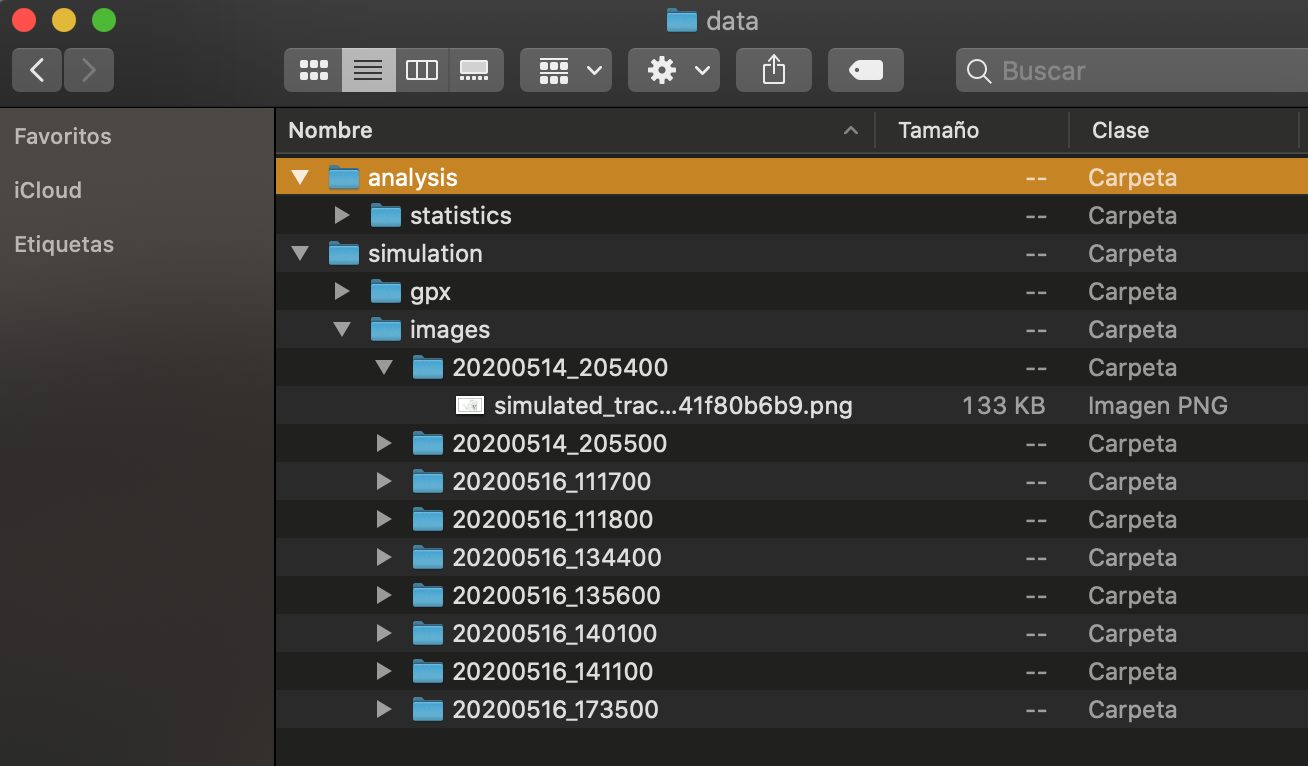
\includegraphics[width=0.95\textwidth]{./Imagenes/dataFolderHierarchy.png}
\caption{Jerarquía en el directorio \textit{\slash track-simulator\slash data}.}
\end{center}
\label{figure:dataFolderHierarchy}
\end{figure}
\newpage

\subsection{Guía de uso}
La interfaz se despliega mediante el uso del comando \textbf{\textit{ts-cli}}. Si no se le 
introduce ningún parámetro se desplegará la ayuda de forma que aparecen las  
acciones disponibles con una pequeña explicación. Las acciones disponibles en la 
primera versión de la herramienta son las siguientes:

\begin{enumerate}[label={A.\arabic*.}]
\item \textbf{analyze}. La acción \textit{analyze} realiza una simulación de una 
trayectoria. Tiene una serie de parámetros de entrada que permiten la personalización 
de su comportamiento.
\begin{enumerate}[label*={P.\arabic*.}]
\item \textbf{file\_directory} Directorio de donde se realizará la lectura de los ficheros 
\ac{GPX} para su análisis. Parte de una ruta inicial \textit{track-simulator/data/analysis}.
\item \textbf{--north\_component} Componente norte del área a analizar.
\item \textbf{--south\_component} Componente sur del área a analizar.
\item \textbf{--east\_component} Componente este del área a analizar.
\item \textbf{--west\_component} Componente oeste del área a analizar.
\end{enumerate}
Si alguno de los parámetros que definen el área de análisis no está definido se usará 
por defecto el territorio delimitado del Castell de Bellver (Mallorca).

\item \textbf{simulate}. La acción \textit{simulate} realiza una simulación de una 
trayectoria. Tiene una serie de parámetros de entrada que permiten la personalización 
de su comportamiento.

\begin{enumerate}[label*={P.\arabic*.}]
\item \textbf{--distance} Distancia que se quiere simular (en metros).

\item \textbf{--origin\_node} Nodo origen desde el que se desea simular la trayectoria.  
El identificador es extraído de la información de \ac{OSM}. Los nodos a destacar para el 
inicio de la trayectoria pueden ser los nodos de entrada al recinto del castillo de Bellver, 
en este caso los siguientes nodos:
\begin{enumerate}
\item 293027796: Entrada noreste.
\item 560055784: Entrada sureste.
\item 317813584: Entrada norte.
\end{enumerate}

\item \textbf{--data}. Conjunto de datos origen que se usarán para la simulación. (Por 
defecto se usará los datos con fecha más reciente). Los datos de MongoDB se guardan 
con formato Graph\_Analysis\_mm-dd-YYYY.

\item \textbf{--quantity}. Número de trayectorias a simular. (Por defecto este valor es 
1).
\end{enumerate}
\end{enumerate}

Se puede utilizar el comando \ref{comand:Help} para observar la lista de para observar 
la lista de parámetros de una acción en concreto.

\begin{lstlisting}[caption={Ejecución ayuda de comando}, language=bash, 
label={comand:Help}] 
	ts-cli analyze [COMMAND] --help
\end{lstlisting}

En el comando \ref{comand:Analyze} se tiene un ejemplo de utilización de la 
herramienta para analizar una conjuntos de trayectorias situadas en la carpeta 
\textit{01-bellver}.

\begin{lstlisting}[caption={Ejecución análisis}, language=bash, 
label={comand:Analyze}] 
	ts-cli analyze --file_directory 01-bellver
\end{lstlisting}

Cabe destacar que la carpeta \textit{01-bellver} tiene que estar situada en el directorio 
\textit{track-simulator/analysis}. Como resultado de esta ejecución se tiene un 
conjunto de datos almacenados dentro de colecciones de la base datos. Junto a esto, 
se pueden observar resultados en la carpeta \textit{track-simulator/data/
analysis/statistics} como muestra la figura \ref{figure:StatisticsFolder}.

\begin{figure}[!htb]
\begin{center}
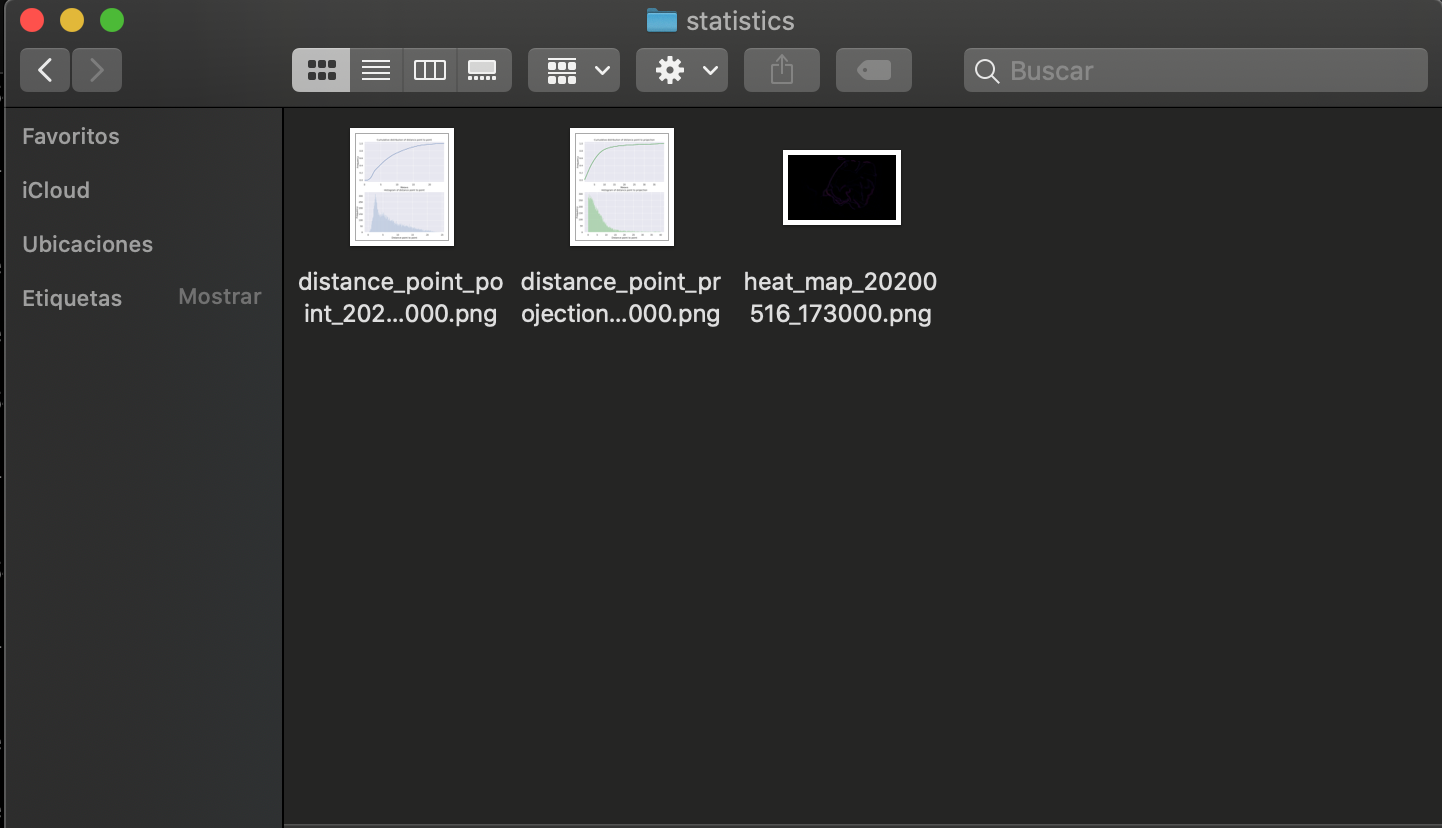
\includegraphics[width=0.95\textwidth]{./Imagenes/statisticsFolderResults.png}
\caption{Directorio \textit{statistics} tras el análisis de un conjunto de trayectorias.}
\label{figure:StatisticsFolder}
\end{center}
\end{figure}
\newpage

Por otro lado,  el comando \ref{comand:Simulate} representa un ejemplo de utilización 
de la herramienta para simular una trayectoria de 10 Kilómetros a partir del análisis 
realizado día 16 de Mayo de 2020.

\begin{lstlisting}[caption={Ejecución simulación}, language=bash, 
label={comand:Simulate}]  
	ts-cli simulate --distance 10000 --data Graph_Analysis_05-16-2020
\end{lstlisting}

Se tiene como resultados de la ejecución un conjunto de trayectorias, tanto ficheros 
\ac{GPX} como un conjunto de imágenes representativas, que serán almacenadas en la 
ruta \textit{track-simulator/data/simulation} como muestra la figura \ref{figure:SimulationFolder}.
\begin{figure}[!htb]
\begin{center}
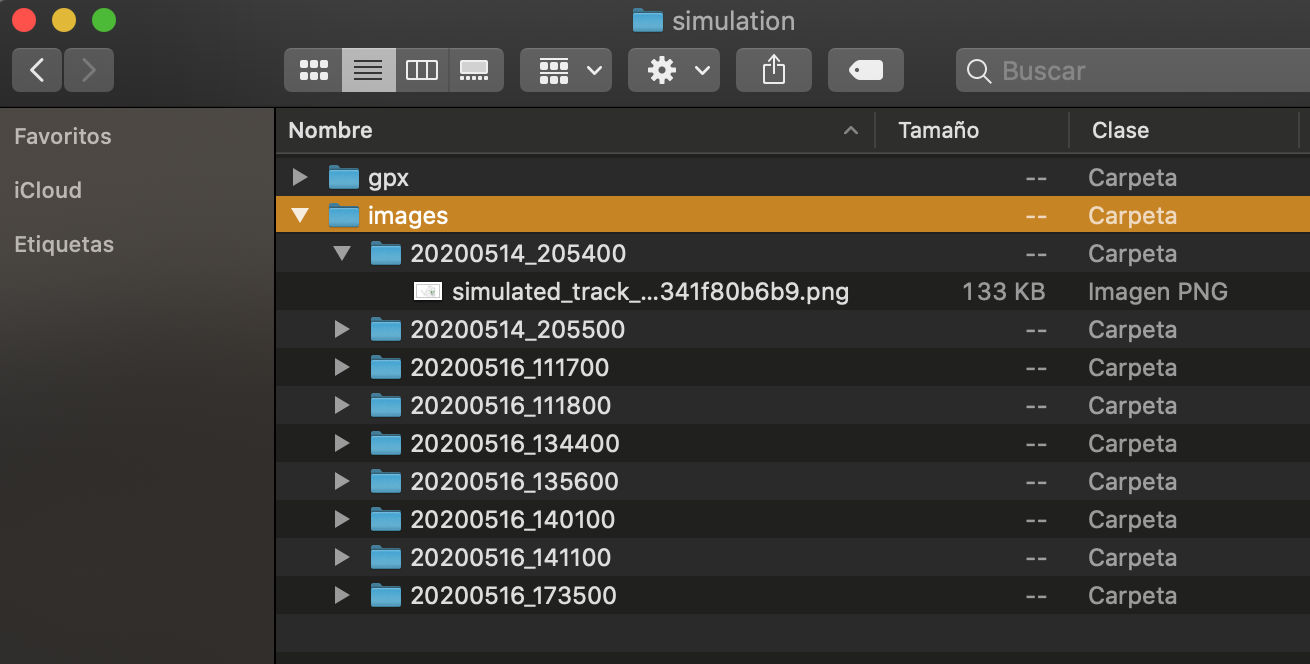
\includegraphics[width=0.8\textwidth]{./Imagenes/SimulationFolderResults.png}
\caption{Directorio \textit{simulation} tras la simulación de un conjunto de trayectorias.}
\label{figure:SimulationFolder}
\end{center}
\end{figure}
\newpage

Se entiende que esta aplicación puede ser utilizada por un público que no tiene 
experiencia en gestion de contenedores Docker, por este motivo, para eliminar los 
recursos utilizados para el procedimiento, por cada uso de la herramienta se 
despliegan y apagan los componentes. Esto supone un tiempo mayor de ejecución, no 
obstante se cree necesario para evitar que los recursos no sean cerrados una vez las 
necesidades del usuario de la aplicación se vean completas.